\documentclass[../Marcus.tex]{subfiles}

\begin{document}

\chapter{Galois Theory Applied to Prime Decomposition}

\subsection*{Exercise 4.1}

Let $\sigma\in D(Q/P)$ and $\tau\in E(Q/P)$ be given. Then for each $\alpha\in S$, we have $\tau\sigma^{-1}(\alpha)\equiv \sigma^{-1}(\alpha) \pmod{Q}$, i.e., $\tau\sigma^{-1}(\alpha)-\sigma^{-1}(\alpha)\in Q$. So $\sigma(\tau\sigma^{-1}(\alpha)-\sigma^{-1}(\alpha))=\sigma\tau\sigma^{-1}(\alpha)-\alpha \in Q$. This means $\sigma\tau\sigma^{-1}(\alpha) \equiv \alpha \pmod{Q}$ and hence $\sigma\tau\sigma^{-1}\in E(Q/P)$.

\subsection*{Exercise 4.2}

Note that $PS=PS_DS_ES=(P'_1\cdots P'_r)S_ES=(P''_1\cdots P''_r)S$. And since $PS=(Q_1\cdots Q_r)^e$, so by the uniqueness of prime decompositions, we have $P''_iS=Q_i^e$ for all $i=1,\ldots,r$. (After rearranging appropriately, of course.)

\subsection*{Exercise 4.3}

(a) Let $g$ be a generator of $(\ZZ/p\ZZ)^\times$. Consider the equation $x^2\equiv -1\pmod{p}$. Write $x=g^k,1\leq k\leq p-1$, and $-1=g^{(p-1)/2}$, then $g^{2k}\equiv g^{(p-1)/2}\pmod{p}$. If it has solutions, then we must have $(p-1)/2\mid 2k$. So the only possible solutions to $k$ are $(p-1)/4$ and $3(p-1)/4$. And these two are integers if and only if $p\equiv 1\pmod{4}$. This completes the proof.

Note that since $(\ZZ/p\ZZ)^\times=\{g,g^2,g^3,\ldots,g^{p-1}\}$, so the squares in $(\ZZ/p\ZZ)^\times$ are precisely $\{g^2,g^4,g^6,\ldots,g^{p-1}\}$. This means for $g^n\in(\ZZ/p\ZZ)^\times$, $(g^n/p)=1$ if and only if $n$ is even. So if we write $a=g^s,b=g^t$ and $ab=g^{s+t}$. Then $(ab/p)=1 \iff s+t$ is even $\iff s,t$ have the same parity $\iff (a/p)=(b/p)$. Hence, $(a/p)(b/p)=(ab/p)$.

(b) First, consider the case where $q=2$. This is easily seen by using Theorem 25 (p. 52). So $(2/p)=1 \iff$ $2$ splits completely in $\QQ(\sqrt{\pm p}) \iff \pm p\equiv 1 \pmod{8} \iff p\equiv \pm1 \pmod{8}$.

Now, assume $q\neq p$ is an odd prime. We split it into three cases and use Theorem 25 again.

Case 1: $p\equiv 1\pmod{4}$. Then $(q/p)=1 \iff$ $q$ splits completely in $\QQ(\sqrt{p}) \iff$ $p$ is a square mod $q$ $\iff (p/q)=1$. So we have $(q/p)=(p/q)$.

Case 2: $p\equiv 3\pmod{4}$ and $q\equiv 1\pmod{4}$. Then $(q/p)=1 \iff$ $q$ splits completely in $\QQ(\sqrt{-p}) \iff$ $-p$ is a square mod $q$ $\iff (-p/q)=1 \iff (-1/q)(p/q)=(p/q)=1$. So we have $(q/p)=(p/q)$. (We've used (a) in the last step.)

Case 2: $p\equiv q \equiv3\pmod{4}$. Then $(q/p)=1 \iff$ $q$ splits completely in $\QQ(\sqrt{-p}) \iff$ $-p$ is a square mod $q$ $\iff (-p/q)=1 \iff (-1/q)(p/q)=-(p/q)=1$. So we have $(q/p)=-(p/q)$. (We've again used (a) in the last step.)

\subsection*{Exercise 4.4}

For (a), (b), (c) and (d), write $b=\prod p_i^{r_i}$ and $b'=\prod q_j^{s_j}$.

(a) From Exercise 4.3(a), we know $(a/p)(b/p)=(ab/p)$ when $p$ is an odd prime. For the first one,
\begin{align*}
    \left(\dfrac{aa'}{b}\right) &= \left(\dfrac{aa'}{\prod p_i^{r_i}}\right) \overset{\df}{=} \prod\left(\dfrac{aa'}{p_i}\right)^{r_i} \\
    &= \prod \left(\dfrac{a}{p_i}\right)^{r_i}\left(\dfrac{a'}{p_i}\right)^{r_i}
    \overset{\df}{=} \left(\dfrac{a}{\prod p_i^{r_i}}\right)\left(\dfrac{a'}{\prod p_i^{r_i}}\right) = \left(\dfrac{a}{b}\right)\left(\dfrac{a'}{b}\right)
\end{align*}
And for the second one,
\begin{align*}
    \left(\dfrac{a}{bb'}\right) &= \left(\dfrac{a}{\prod p_i^{r_i}\prod q_j^{s_j}}\right) \overset{\df}{=} \prod\left(\dfrac{a}{p_i}\right)^{r_i}\prod\left(\dfrac{a}{q_j}\right)^{s_j} \\
    &\overset{\df}{=} \left(\dfrac{a}{\prod p_i^{r_i}}\right)\left(\dfrac{a}{\prod q_j^{s_j}}\right) = \left(\dfrac{a}{b}\right)\left(\dfrac{a}{b'}\right)
\end{align*}

(b) We know $(a/p)=(a'/p)$ for Legendre symbols if $a\equiv a'\pmod{p}$. Note that if $a\equiv a'\pmod{b}$, then $a\equiv a'\pmod{p_i}$ for all $i$. So $(a/b)\overset{\df}{=}\prod (a/p_i)^{r_i}=\prod (a'/p_i)^{r_i}\overset{\df}{=}(a'/b)$.

(c) Let $p_1,\ldots,p_n$ be all prime divisors of $b$ of the form $4k+3$. This means the Legendre symbol $(-1/p_i)=-1$ for all $i=1,\ldots,n$. The result now follows from the observation that $(-1/b)\overset{\df}{=}\prod (-1/p_i)^{r_i}=1 \iff \#\{r_1,\ldots,r_n \text{ is odd}\}$ is even $\iff b=\prod p_i^{r_i}\equiv 1\pmod{4}$.

(d) Let $p_1,\ldots,p_n$ be all prime divisors of $b$ of the form $8k\pm3$. This means the Legendre symbol $(2/p_i)=-1$ for all $i=1,\ldots,n$. The result now follows from the observation that $(2/b)\overset{\df}{=}\prod (2/p_i)^{r_i}=1 \iff \#\{r_1,\ldots,r_n \text{ is odd}\}$ is even $\iff b=\prod p_i^{r_i}\equiv \pm1\pmod{8}$.

(e) Write $a=\prod p_i$ where $p_i$ not necessarily distinct and $b=\prod q_j$ also not necessarily distinct. Observe that $(a/b)(b/a)\overset{(a)}{=}\prod (p_i/q_j)(q_j/p_i)=(-1)^k$ where $k$ is the number of pairs where $p_i$ and $q_j\equiv 3\pmod{4}$. Moreover, $(-1)^k=(-1)^{mn}$ where $m$ and $n$ are the numbers of $p_i$ and $q_j\equiv 3\pmod{4}$, respectively. Note that $(-1)^{mn}=1 \iff$ at least one of $m,n$ is even $\iff$ at least one of $a,b\equiv 1\pmod{4}$. This shows that $(a/b)(b/a)=1 \iff$ at least one of $a,b\equiv 1\pmod{4}$, which completes the proof.

(f) We don't need to bother factoring $2413$, just simply apply the results we have shown. (In fact, $2413 = 19\times 127$.)
\begin{align*}
    \left(\dfrac{2413}{4903}\right) &\overset{(e)}{=} \left(\dfrac{4903}{2413}\right) \overset{(b)}{=} \left(\dfrac{77}{2413}\right) \overset{(a)}{=} \left(\dfrac{7}{2413}\right)\left(\dfrac{11}{2413}\right) \\ &\overset{(e)}{=} \left(\dfrac{2413}{7}\right)\left(\dfrac{2413}{11}\right) \overset{(b)}{=} \left(\dfrac{5}{7}\right)\left(\dfrac{4}{11}\right) = -1
\end{align*}

\subsection*{Exercise 4.5}

We use the same notation as in the textbook. (See Theorem 28 (p. 70) and Theorem 29 (p. 73). These two are also the main results we are going to use.) For the followings, we fix a prime $Q$ in $L$.

(a) Suppose $P$ is inert in $L$. This means $r=e=1$ and so $L_D = K$ and $L=L_E$. By Galois theory, we have $D=G$ and $E = \{\id_L\}$. Hence, $D/E=G/\{\id_L\}\simeq G$ is cyclic by Corollary 1 (p. 71).

(b) Suppose there's an intermediate field $K\sbne K'\sbne L$. Let $P'$ be the unique prime in $K'$ lying under $Q$, then $P'$ also lies over $P$. As $P$ is totally ramified in $K'$, we have $e(P'/P)=[K':K]>1$.

We consider the inertia field $L_E$.

Case 1: If $L_E=L$. Then we have $e=1$ and so $e(P'/P)=1$, a contradiction.

Case 2: If $L_E=K$. Then $e=[L:K]$ and so $P$ is totally ramified in $L$, a contradiction.

Case 3: If $L_E$ is an intermediate field. Then by assumption $P$ is totally ramified in $L_E$. So $1=e(Q_E/P)=[L_E:K]$, a contradiction. 

We may conclude that there's no intermediate field between $K$ and $L$. And so by Galois theory, there's no non-zero proper subgroup in $G$. This implies that $G$ is cyclic of prime order. (If not, then by Sylow theorem, there would be a non-zero proper subgroup.)

(c) Suppose there's an intermediate field $K\sbne K'\sbne L$. Let $P'$ be the unique prime in $K'$ lying under $Q$, then by assumption, $P'$ is the unique prime in $K'$ lying over $P$.

We consider the decomposition field $L_D$.

Case 1: If $L_D=L$. Then we have $e=f=1$ and so $e(P'/P)=f(P'/P)=1$. This implies $[K':K] = e(P'/P) \cdot f(P'/P) = 1$, a contradiction.

Case 2: If $L_D=K$. Then $r=1$ and so $Q$ is the only prime in $L$ lying over $P$, a contradiction.

Case 3: If $L_D$ is an intermediate field. Then by assumption $Q_D$ is the only prime in $L_D$ lying over $P$. So $[L_D:K]=e(Q_D/P)f(Q_D/P)=1$, a contradiction.

We may again conclude that there's no intermediate field between $K$ and $L$. So similar to (b), this implies $G$ is cyclic of prime order.

(d) First note that if there are no intermediate fields $K\sbne K'\sbne L$, then by Galois theory, the only subgroups of $G$ are $\{\id_L\}$ and $G$. In this case, take $H=G$ and done.

Now, assume there's at least one intermediate field $K'$. Then for each such $K'$, by assumption we have $e(P'/P)=1$ for each $P'$ in $K'$ lying over $P$. So by Theorem 29 (3), $K'\sbe L_E$. This shows $L_E$ contains all intermediate fields. Moreover, since $P$ is ramified in $L$, so $L_E\sbne L$. Hence by Galois theory, the corresponding subgroup $E$ is the smallest non-trivial subgroup in $G$. (The uniqueness is clear.)

Note that for any $g\in G$, since $gEg^{-1}$ and $g^{-1}Eg$ are also subgroups of $G$, so we have $E \sbe gEg^{-1}$ and $E \sbe g^{-1}Eg$. These two imply that $gE=Eg$, i.e., $E$ is normal in $G$.

Let's show $G$ and $H=E$ have the desired properties. If there are distinct primes $p,q$ s.t. $p,q \mid \#(G)$, then by Cauchy's theorem, $\exists a,b\in G$ with order $p,q$, respectively. Since $H$ is the smallest subgroup, $H \sbe \langle a \rangle,\langle b \rangle$. This implies $\#(H)\mid p,q$ and so $\#(H)=1$, which is absurd. So $\#(G)$ is a prime power. Consequently, $H$ must have prime order. Lastly, since $G$ has non-trivial center, so $H\sbe Z(G)$.

(e) Similar to (d), we assume there's at least one intermediate field $K'$. For each such $K'$, by assumption we have $e(P'/P)=f(P'/P)=1$ for each $P'$ in $K'$ lying over $P$. So by Theorem 29 (1), $K'\sbe L_D$. This shows $L_D$ contains all intermediate fields. Moreover, since $P$ does not split completely in $L$, so $L_D\sbne L$. Hence by Galois theory, the corresponding subgroup $D$ is the smallest non-trivial subgroup in $G$. (The uniqueness is clear.) The rest are the same as (d).

As an example, let $K=\QQ$ and $L=\QQ(e^{2\pi i/5})$. We know $G=(\ZZ/5\ZZ)^\times\simeq C_4$, the cyclic group of order $4$. There's only one non-trivial proper subgroup in $C_4$, namely, $\{0,2\}$. So by Galois correspondence, there's only one intermediate field. Moreover, by Exercise 2.8, we know this field is $\QQ(\sqrt{5})$. Note that the corresponding subgroup $H$ is isomorphic to $\{0,2\}$, which clearly has the desired properties.

Consider $p=11$. Since $5$ is a square mod $11$, by Theorem 25 (p. 52), we have $11$ splits completely in $\QQ(\sqrt{5})$. Moreover, by Theorem 26 (p. 53), $f=2$ is the order of $11$ in $(\ZZ/5\ZZ)^\times$. So $11$ does not split completely in $L=\QQ(e^{2\pi i/5})$.

(f) Suppose $P$ is inert in every intermediate field $K'$. Note the condition on $L$ implies that $r>1$ or $e>1$. If $r>1$, then the assumption in (c) is satisfied. So $G$ is cyclic of prime order.

Assume $e>1$, then the assumption in (d) is satisfied. So $\#(G)=p^m$. And $E$ is the unique smallest non-trivial subgroup in $G$. Note that if $K\sbne L_D$, then $L_D$ is an intermediate field. By assumption $P$ is inert in $L_D$. So $1 = f(Q_D/P) = [L_D:K]$, a contradiction. This shows $K=L_D$ and so $G=D$.

From (d) we know $E=H\sbe Z(G)\sbe G=D$. By the third isomorphism theorem, $G/Z(G) \simeq (G/H)/(Z(G)/H) = (D/E)/(Z(G)/E)$. From Corollary 1 (p. 71) we know  $D/E$ is cyclic. In particular, so is $G/Z(G)$. Thus by group theory we have $G$ is abelian. And the fundamental theorem of finite abelian groups tells us $G$ is a direct sum of cyclic groups of prime power order. Then since $\#(G)=p^m$, we must have $G\simeq \ZZ/p^m\ZZ$ is cyclic.

\subsection*{Exercise 4.6}

By Exercise 2.42, $K$ contains $\QQ(\sqrt{k})$ where $k:=mn/\gcd(m,n)^2$. This is the third quadratic subfield.

Note that since $G$ is abelian, by the remark in page 76, we know the groups $D$ and $E$ are independent of the primes in $K$ lying over $p$. Also note that the corresponding fields $K_D$ and $K_E$ have only five candidates, namely, $\QQ,\QQ(\sqrt{m}),\QQ(\sqrt{n}),\QQ(\sqrt{k})$ and $K$.

The main results we are going to use are Theorem 28 (p. 70) and Theorem 29 (p. 73). All the splittings of a given prime $p$ in the quadratic fields can be found in Theorem 25 (p. 52). In addition, we know $4=[K:\QQ]=ref$.

(a) Since $p$ is ramified in each of the quadratic subfields, so $p$ splits into a square of single prime in these fields. By Theorem 29 (3), $K_E$ cannot be any of these quadratic subfields, let alone $K$. This implies $K_E=\QQ$. So $e=4$ and $f=r=1$, i.e., $p$ splits into $P^4$ in $K$.

As an example, consider $n=2,m=3$ and $p=2$, then $2$ is ramified in $\QQ(\sqrt{2}),\QQ(\sqrt{3})$ and $\QQ(\sqrt{6})$. So $2$ splits into $P^4$ in $K=\QQ(\sqrt{2},\sqrt{3})$.

(b) Suppose $p$ splits completely in each of the quadratic subfields, then by Theorem 29 (1), $K_D$ contains all these fields. This implies $K_D=K$. So $r=4$ and $e=f=1$, i.e., $p$ splits completely in $K$.

As an example, consider $n=-2,m=7$ and $p=3$, then $3$ splits completely in $\QQ(\sqrt{-2}),$ $\QQ(\sqrt{7})$ and $\QQ(\sqrt{-14})$. So $3$ splits completely in $K=\QQ(\sqrt{-2},\sqrt{7})$.

(c) Suppose $p$ is inert in each of the quadratic subfields, this forces $f\geq 2$. Moreover, by Theorem 29 (3), $K_E$ contains all these fields. This implies $K_E=K$ and so $e=1$.

If $f=2$, then $r=2$, $K_D$ is a quadratic field. So $p$ is inert in $K_D$, which is impossible because we know the corresponding ramification index and inertial degree must be $1$. On the other hand, if $f=4$, then $r=1=e$, $p$ is inert in $K$. By Exercise 4.5 (a), we have $G$ is cyclic, which is a contradiction. So we may conclude that this case can't occur.

(d) For $p$ splits into $PQ$ in $K$, this means $r=f=2$ and $e=1$. Take $n=2,m=7$ and $p=3$. Since $3$ is inert in $\QQ(\sqrt{2})$, we have $f\geq 2$. And since $3$ splits into two primes in $\QQ(\sqrt{7})$, we have $r\geq 2$. From these two we may conclude that in fact $r=f=2$ and $e=1$.

For $p$ splits into $(PQ)^2$ in $K$, this means $r=e=2$ and $f=1$. Take $n=2,m=-7$ and $p=2$. Since $2$ splits into a square in $\QQ(\sqrt{2})$, we have $e\geq 2$. And since $2$ splits into two primes in $\QQ(\sqrt{-7})$, we have $r\geq 2$. From these two we may conclude that in fact $r=e=2$ and $f=1$.

For $p$ splits into $P^2$ in $K$, this means $e=f=2$ and $r=1$. Take $n=3,m=5$ and $p=2$. Since $2$ splits into a square in $\QQ(\sqrt{3})$, we have $e\geq 2$. And since $2$ is inert in $\QQ(\sqrt{5})$, we have $f\geq 2$. From these two we may conclude that in fact $e=f=2$ and $r=1$.

\subsection*{Exercise 4.7}

If $K=\QQ(\sqrt{m})$ and $L=\QQ(\sqrt{n})$ where $m,n\neq 1$ are distinct square-free integers, then $KL=\QQ(\sqrt{m},\sqrt{n})$, which is normal over $\QQ$ with degree $4$. And from Exercise 4.6 we know there's another quadratic subfield $\QQ(\sqrt{k})$ where $k:=mn/\gcd(m,n)^2$ contained in $KL$.

All the splittings of a given prime $p$ in the quadratic fields can be found in Theorem 25 (p. 52). In addition, the numbers $r,e,f$ are set to be corresponding to the splitting of $p$ in $KL$.

(a) Take $K=\QQ(\sqrt{-1}),L=\QQ(\sqrt{3})$ and $p=2$. Then $2$ is totally ramified in both $K$ and $L$. Note that since $2$ is inert in $\QQ(\sqrt{k})=\QQ(\sqrt{-3})$, we know $f\geq 2$. So $2$ cannot be totally ramified in $KL$.

(b) Take $K=\QQ(\sqrt{-1}),L=\QQ(\sqrt{7})$ and $p=2$. Then $2$ splits into a square of single prime in both $K$ and $L$. Note that since $2$ splits into two primes in $\QQ(\sqrt{k})=\QQ(\sqrt{-7})$, we know $r\geq 2$. So $KL$ cannot contain a unique prime lying over $2$.

(c) Take $K=\QQ(\sqrt{-3}),L=\QQ(\sqrt{5})$ and $p=2$. Then $2$ is inert in both $K$ and $L$. Note that since $2$ splits into two primes in $\QQ(\sqrt{k})=\QQ(\sqrt{-15})$, we know $r\geq 2$. So $2$ cannot be inert in $KL$.

(d) Take $K=\QQ(\sqrt{-1}),L=\QQ(\sqrt{3})$ and $p=2$. Then $2$ is totally ramified in both $K$ and $L$, so the corresponding inertial degrees are all $1$. Note that since $2$ is inert in $\QQ(\sqrt{k})=\QQ(\sqrt{-3})$, we know $f\geq 2$. So the residue field extension of $\ZZ/2\ZZ$ is not trivial for $KL$.

\subsection*{Exercise 4.8}

(a) For a prime $q$, let $K$ be the $q$-th cyclotomic field. Write $(\ZZ/q\ZZ)^\times=\langle a\rangle$, then $\ord_q(a^r) = (q-1)/r$. Since $\gcd(a^r,q)=1$, by Dirichlet's theorem, we may take a prime $p$ s.t. $p\equiv a^r \pmod{q}$. In particular, $p \nmid q$. So by the Corollary of Theorem 26 (p. 54), $p$ splits into $\phi(q)/f$ distinct primes in $K$, where $f = \ord_q(p) = \ord_q(a^r) = (q-1)/r$. Hence $p$ splits into $\phi(q)/f = r$ distinct primes in $K$.

(b) Similar to (a), but this time we require $q \equiv 1 \pmod{rf}$. Then we still have a prime $p$ that splits into $r$ distinct primes in $K$. And since $G := \Gal(K/\QQ) \simeq (\ZZ/q\ZZ)^\times$ is cyclic of order $q-1$ and $rf \mid q-1$, so there is a (unique) subgroup $H$ of $G$ with $[G:H] = rf$. Then by Galois theory, $K_H$ is a subfield of $K$ with degree $rf$ over $\QQ$.

Since $p$ splits into $r$ distinct primes in $K$, by the remark of Corollary 2 (p. 72), $K_D$ is the unique intermediate field with $[K_D:\QQ]=r$. And since $G$ is cyclic and $r = [G:D] \mid [G:H] = rf$, we know $D \spe H$ and so $K_D \sbe K_H$. By the same remark, this implies $p$ also splits into $r$ distinct primes in $K_H$.

(c) Similar to (a), but this time we require $q \equiv 1 \pmod{ref}$. Note that in particular $\gcd(q,e)=1$. So by Chinese remainder theorem, $(\ZZ/qe\ZZ)^\times \simeq (\ZZ/q\ZZ)^\times \times (\ZZ/e\ZZ)^\times$. We then take $x \in (\ZZ/qe\ZZ)^\times$ s.t. $x\equiv a^r\pmod{q}$ and $x\equiv 1\pmod{e}$. (Recall that $(\ZZ/q\ZZ)^\times=\langle a\rangle$.)

By Dirichlet's theorem again, there is a prime $p \equiv x \pmod{qe}$. Then $p\equiv 1\pmod{e}$ and $p\equiv a^r\pmod{q}$. This $p$ is what we want by (a) and (b).

(d) By (b), there is a subfield $K'$ of the $q$-th cyclotomic field $K$ with $[K':\QQ] = rf$ s.t. $p$ splits into $r$ distinct primes in $K'$. On the other hand, by Theorem 26 (p. 53), $p$ is totally ramified in the $p$-th cyclotomic field $L$. Since $\Gal(L/\QQ)$ is cyclic of order $p-1$ and $e \mid p-1$, so by Galois theory there is a subfield $L'$ of $L$ s.t. $[L':\QQ]=e$. And by Exercise 3.24 (a) we know $p$ is also totally ramified in $L'$.

That is to say, let $P'$ (resp. $Q'$) be a prime in $K'$ (resp. $L'$) lying over $p$. Then we have $e(P'/p) = 1, f(P'/p) = f$, and on the other hand, $e(Q'/p) = e, f(Q'/p) = 1$.

Consider the compositum $K'L'$, which is a subfield of the $pq$-th cyclotomic field $M$. Then we have the following field extensions:
\begin{center}
    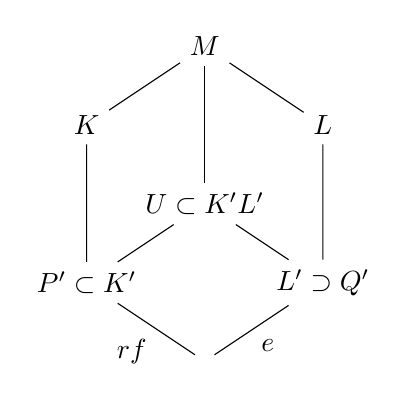
\begin{tikzpicture}
    \draw (0,0) node (Q) {$\QQ$};
    \draw (-1.5,1) node (K') {$P' \subset K'$};
 	\draw (-1.5,3) node (K) {$K$};
	\draw (1.5,1) node (L') {$L' \supset Q'$};
    \draw (1.5,3) node (L) {$L$};
	\draw (0,2) node (K'L') {$U \subset K'L'$};
    \draw (0,4) node (M) {$M$};
    
	\draw (Q) -- node[below left] {$rf$} (K') -- (K) -- (M) -- (L) -- (L') -- (L') -- node[below right] {$e$} (Q);
	\draw (K') -- (K'L') -- (L');
	\draw (K'L') -- (M);
    \end{tikzpicture}
\end{center}
We claim that this $K'L'$ is what we want. Suppose $U$ is a prime in $K'L'$ lying over $p$. Then $U$ also lies over $P'$ and $Q'$. Note that we have
$$
e(U/p) = e(U/Q')e(Q'/p) \geq e \quad \text{and} \quad f(U/p) = f(U/P')f(P'/p) \geq f
$$
Suppose there are $s$ primes in $K'L'$ lying over $p$ (so $s\geq r$), then
$$
ref = [K' : \QQ][L' : \QQ] \geq [K'L' : \QQ] = s \cdot e(U/p) \cdot f(U/p) \geq ref
$$
So everything is an equality. In particular, we have $s=r$, $e(U/p) = e$ and $f(U/p) = f$, as desired.

(e) We follow the procedure given in (c). First, find a prime $q \equiv 1 \pmod{2\cdot3\cdot5}$. We can take $q=31$. Note that $(\ZZ/31\ZZ)^\times = \langle3\rangle$. (In the notation in (c), $a=3$.) Next, we solve the congruence equations
$$
\begin{cases}
x \equiv 3^5 \equiv 26 \pmod{31} \\
x \equiv 1 \pmod{2}
\end{cases}
$$
A simple calculation shows that $x=57$ works. Finally, find a prime $p \equiv 57 \pmod{31\cdot2}$. We can take $p=181$.

\subsection*{Exercise 4.9}

(a) For the decomposition groups,
\begin{align*}
    D' &= D(Q'/P) = D(\sigma(Q)/P) = D(\sigma(Q)/P) \\
	&= \{\tau\in G\mid \tau\sigma(Q)=\sigma(Q)\} = \{\tau\in G\mid \sigma^{-1}\tau\sigma(Q)=Q\} \\
    &= \{\tau\in G\mid \sigma^{-1}\tau\sigma \in D(Q/P)\}   \\
	&= \sigma D(Q/P) \sigma^{-1} = \sigma D\sigma^{-1}
\end{align*}

For the inertia groups,
\begin{align*}
    E' &= E(Q'/P) = E(\sigma(Q)/P) = E(\sigma(Q)/P) \\
	&= \{\tau\in G \mid \tau(\alpha) \equiv \alpha \pmod{\sigma(Q)}, \forall\alpha\in S\} \\
	&= \{\tau\in G \mid \sigma^{-1}\tau(\alpha) \equiv \sigma^{-1}(\alpha) \pmod{Q}, \forall\alpha\in S\} \\
    &= \{\tau\in G \mid \sigma^{-1}\tau\sigma\sigma^{-1}(\alpha) \equiv \sigma^{-1}(\alpha) \pmod{Q}, \forall\alpha\in S\} \\
    &= \{\tau\in G\mid \sigma^{-1}\tau\sigma(\beta) \equiv \beta \pmod{Q}, \forall\beta\in S\} \\
    &= \{\tau\in G\mid \sigma^{-1}\tau\sigma\in E(Q/P)\} \\
    &= \sigma E(Q/P)\sigma^{-1} = \sigma E\sigma^{-1}
\end{align*}

(b) By the uniqueness of Frobenius automorphisms (Theorem 32 (p. 77)), it's sufficient to show that $\sigma\phi\sigma^{-1}$ has the same property with $\phi'$, i.e., $\sigma\phi\sigma^{-1}(\alpha)\equiv\alpha^{\|P\|} \pmod{Q'=\sigma(Q)}$ for all $\alpha\in S$. But notice that
\begin{align*}
    &\sigma\phi\sigma^{-1}(\alpha)\equiv\alpha^{\|P\|} \pmod{\sigma(Q)}, \forall\alpha\in S \\
    \iff{} &\phi\sigma^{-1}(\alpha) \equiv \sigma^{-1}(\alpha)^{\|P\|} \pmod{Q}, \forall\alpha\in S \\
    \iff{} &\phi(\beta) \equiv \beta^{\|P\|} \pmod{Q}, \forall\beta\in S
\end{align*}
Since the last statement holds, the result follows.

\subsection*{Exercise 4.10}

(a) Let $\sigma\in D(V/Q)\sbe\Gal(LM/L)$, then $\sigma(V)=V$. Observe that $\sigma|_M(U)=\sigma|_M(V\cap M)=\sigma(V\cap M)=\sigma(V)\cap\sigma(M)=V\cap\sigma|_M(M)=V\cap M=U$, so $\sigma|_M\in D(U/P)$.

(b) Let $\sigma\in E(V/Q)\sbe\Gal(LM/L)$, then $\sigma(\alpha)\equiv\alpha \pmod{V}$ for all $\alpha\in \AA \cap LM$. For any $\alpha\in \AA \cap M$, we know $\sigma|_M(\alpha)-\alpha\in M$. On the other hand, since $\alpha\in \AA \cap M \subset \AA \cap LM$, we have $\sigma|_M(\alpha)-\alpha=\sigma(\alpha)-\alpha\in V$. So $\sigma|_M(\alpha)-\alpha\in M\cap V=U$ and hence $\sigma|_M(\alpha)\equiv\alpha\pmod{U}$. So $\sigma|_M\in E(U/P)$.

(c) Since $e(U/P)=1$, by Theorem 28 (p. 70), we have $E(U/P)=\{\id_M\}$. By (b) we know $E(V/Q)|_M:=\{\sigma|_M \mid \sigma\in E(V/Q)\} \sbe E(U/P)=\{\id_M\}$, so $\sigma|_M=\id_M$ for all $\sigma\in E(V/Q)$. This means $M$ is fixed by all elements in $E(V/Q)$. Moreover, since $L$ is necessarily fixed by these elements, we have $E(V/Q)=\{\id_{LM}\}$, which implies $e(V/Q)=1$.

(d) Similar to (c), since $e(U/P)=f(U/P)=1$, by Theorem 28 again, we have $D(U/P)=\{\id_M\}$. By (a) we know $D(V/Q)|_M:=\{\sigma|_M \mid \sigma\in D(V/Q)\} \sbe D(U/P)=\{\id_M\}$, so $\sigma|_M=\id_M$ for all $\sigma\in D(V/Q)$. This means $M$ is fixed by all elements in $D(V/Q)$. Moreover, since $L$ is necessarily fixed by these elements, we have $D(V/Q)=\{\id_{LM}\}$, which implies $e(V/Q)=f(V/Q)=1$.

(e) Since $P$ is unramified in $M$, we know $D(U/P)$ is isomorphic to the Galois group of $(\AA \cap M)/U$ over $(\AA \cap K)/P$. So if two maps $\phi(V/Q)|_M$ and $\phi(U/P)^{f(Q/P)}$ in $D(U/P)$ induce the same map in the Galois group, then they are necessarily the same. 

Let $\ovl{\phi}(V/Q)|_M$ be the map induced from $\phi(V/Q)|_M$. Note that $\ovl{\phi}(V/Q)$ generates the Galois group of $(\AA \cap LM)/V$ over $(\AA \cap L)/Q$ and maps an element in $(\AA \cap LM)/V$ to its $\|Q\|$ power. Now, view $(\AA \cap LM)/V$ as a field extension of $(\AA \cap M)/U$. Then for each $x+U \in (\AA \cap M)/U$, we have
$$
\ovl{\phi}(V/Q)|_M(x+U)=\ovl{\phi}(V/Q)(x+U)=(x+U)^{\|Q\|}=x^{\|Q\|}+U
$$

On the other hand, let $\ovl{\phi}(U/P)$ be the map induced from $\phi(U/P)$. Note that $\ovl{\phi}(U/P)$ generates the Galois group of $(\AA \cap M)/U$ over $(\AA \cap K)/P$ and maps an element in $(\AA \cap M)/U$ to its $\|P\|$ power. So for each $x+U \in (\AA \cap M)/U$, we have
$$
\ovl{\phi}(U/P)^{f(Q/P)}(x+U)=x^{\|P\|^{f(Q/P)}}+U
$$

Consider the field extension $(\AA \cap L)/Q$ over $(\AA \cap K)/P$ with degree $f(Q/P)$, then we have $\|Q\|=\|P\|^{f(Q/P)}$. This implies that $\ovl{\phi}(V/Q)|_M=\ovl{\phi}(U/P)^{f(Q/P)}$, as desired.

\subsection*{Exercise 4.11}

(a) Suppose $K\subset L\subset M$ and $M$ is normal over $K$, then $LM=M$. (So $V=U$.) Then by Exercise 4.10 (e), we have $\phi(V/Q)|_M=\phi(U/Q)=\phi(U/P)^{f(Q/P)}$.

(b) By the uniqueness of Frobenius automorphisms (Theorem 32 (p. 77)), it's sufficient to show that $\phi(U/P)|_L$ has the same property with $\phi(Q/P)$, i.e., $\phi(U/P)|_L(\alpha)\equiv\alpha^{\|P\|} \pmod{Q}$ for all $\alpha\in \AA \cap L$. Fix such $\alpha$, we know $\phi(U/P)|_L(\alpha)-\alpha^{\|P\|}\in L$. On the other hand, since $\alpha\in \AA \cap L \subset \AA \cap M$, we have $\phi(U/P)|_L(\alpha)-\alpha^{\|P\|}=\phi(U/P)(\alpha)-\alpha^{\|P\|}\in U$. So $\phi(U/P)|_L(\alpha)-\alpha^{\|P\|} \in L\cap U=Q$ and hence $\phi(U/P)|_L(\alpha)\equiv\alpha^{\|P\|} \pmod{Q}$.

\subsection*{Exercise 4.12}

(a) Since $K/\QQ$ is normal and $p$ is unramified in $K$ (as $p$ is unramified in $\QQ(\omega)$), we can consider the Frobenius automorphism $\phi(P/p)$. Let $Q$ be a prime in $\QQ(\omega)$ lying over $P$. From Exercise 4.11 (b), we know $\phi(P/p)=\phi(Q/p)|_K$. Since $f(P/p)$ is the order of $\phi(P/p)$, we have $f(P/p)$ is the least positive integer s.t. $\phi(P/p)^{f(P/p)}=\id_K$. So $f(P/p)$ is the least positive integer s.t. $\phi(Q/p)^{f(P/p)}$ fixes $K$ pointwise, which means $\phi(Q/p)^{f(P/p)} \in \Gal(\QQ(\omega)/K) \simeq H$.

Note that $\phi(Q/p)$ is the automorphism which maps $\omega$ to $\omega^p$ (see p. 77), so $\phi(Q/p)$ corresponds to the element $p\in(\ZZ/m\ZZ)^\times$. Hence, we have $f(P/p)$ is the least positive integer s.t. $\ovl{p^{f(P/p)}}\in H$, which by definition, is $f$. So $f=f(P/p)$.

Alternatively, we can use Theorem 33 (p. 78) to obtain the same result. Consider $p$ acts on the right coset space of $H$ in $G$. The orbit of $H$ is $\{H,Hp,\ldots,Hp^{f-1}\}$. So by Theorem 33, $f(P/p)=f$.

(b) Let $K:=\QQ(\omega+\omega^{-1})$. For $\sigma\in\Gal(\QQ(\omega)/\QQ)$, write $\sigma(\omega)=\omega^k$ where $\gcd(k,m)=1$. We want to find all $k\in(\ZZ/m\ZZ)^\times$ s.t. $\sigma(\omega+\omega^{-1})=\omega^k+\omega^{-k}=\omega+\omega^{-1}$. It's easy to see that $1,-1\in(\ZZ/m\ZZ)^\times$ are two solutions. Moreover, by Exercise 2.35 (b), $[\QQ(\omega):K]=2$, so by Galois correspondence, $\#(H)=2$. Hence we have $H=\{1,-1\}\subset(\ZZ/m\ZZ)^\times$.

Let $f$ be the least positive integer s.t. $p^f \equiv \pm1\pmod{m}$, then by (a), $f(P/p)=f$. Hence $p$ splits into $[K:\QQ] / f = \phi(m)/(2f)$ primes in $K$.

(c) Note that $\ovl{p}\in H \iff f = 1$. And by (a), $f(P/p)=f$. So $\ovl{p}\in H \iff f(P/p) = 1 \iff p$ splits into two primes in $\QQ(\sqrt{d})$. By Theorem 25 (p. 52), if $p$ is odd, then this is equivalent to say that $d$ is a square mod $p$. And if $p=2$, then this is equivalent to say that $d\equiv 1\pmod{8}$.

\subsection*{Exercise 4.13}

(a) Note that $K:=\QQ(\alpha)$ and $K':=\QQ(i)$ are two intermediate fields, so by Galois theory, $H:=\Gal(L/K)$ and $H':=\Gal(L/K')$ are two subgroups of $G$.
For $H$, we know $\#(H)=[L:K]=2$. Define $\tau$ by $\tau(\alpha)=\alpha$ and $\tau(i)=-i$, then $\tau|_K=\id_K$. From this it's easy to see that $H=\{\id_L,\tau\}$. Note that $\tau$ represents the permutation $(24)$.

On the other hand, we know $\#(H')=[L:K']=4$. Define $\sigma$ by $\sigma(\alpha)=i\alpha$ and $\sigma(i)=i$, then $\sigma|_{K'}=\id_{K'}$ and so $\sigma\in H'$. Since $\ord(\sigma)=4$, we have $H'=\langle\sigma\rangle$. Note that $\sigma$ represents the permutation $(1234)$.

Since $H\cdot H'\sbe G$ and $\#(G)=8$, we have $G=\{1,\tau,\sigma,\tau\sigma,\sigma^2,\tau\sigma^2,\sigma^3,\tau\sigma^3\}\simeq D_4$, the dihedral group of order $8$.

(b) By the Corollary of Theorem 31 (p. 76), it's enough to show that $p$ is unramified in $K$. To do this, we use Corollary 1 of Theorem 24 (p. 51). Let $f(x)=x^4-m$, then $\Nr(f'(\alpha))=\Nr(4\alpha^3)=4^4\Nr(\alpha)^3=-256m^3$. Since we have $p\nmid -256m^3$, so $p$ is unramified in $K$. 

(c) The right coset space of $H=\Gal(L/K)$ in $G$ is $\{H,H\sigma,H\sigma^2,H\sigma^3\}$. And a simple calculation shows that the action of $\phi(Q/p)=\tau$ on this space gives us three orbits: $\{H\},\{H\sigma,H\sigma\tau=H\tau\sigma^3=H\sigma^3\},\{H\sigma^2\}$. (One may use the fact that $(\tau\sigma)^2=(1)$.) So by Theorem 33 (p. 78), $p$ splits into three primes in $K$.

(d) It's easy to check all the cases. If $\phi=1=\id_L$, there are four orbits, so $p$ splits completely in $K$. If $\phi=\sigma,\sigma^3$, there is only one orbit, so $p$ is inert in $K$. If $\phi=\tau\sigma,\sigma^2,\tau\sigma^3$, there are two orbits. And finally, if $\phi=\tau\sigma^2$, there are three orbits.

\subsection*{Exercise 4.14}

\subsection*{Exercise 4.15}

Suppose there exist distinct automorphisms $\sigma_1,\ldots,\sigma_n$ and $a_1,\ldots,a_n\in F$ not all zero s.t. $\sum a_i\sigma_i = \mathbf{0}$ (the zero map). We may assume $n$ is minimal. Fix $x\in F$ s.t. $\sigma_1(x)\neq\sigma_n(x)$. Note that for each $y\in F$, we have $0 = \sum a_i\sigma_i(xy) = \sum a_i\sigma_i(x)\sigma_i(y)$. So $\sum a_i\sigma_i(x)\sigma_i=\mathbf{0}$. On the other hand, we clearly have $\sum a_i\sigma_1(x)\sigma_i=\mathbf{0}$. Subtracting these two gives us $\sum a_i(\sigma_i(x)-\sigma_1(x))\sigma_i=\mathbf{0}$. Note that we have $1\leq\#(\text{terms})<n$ because $\sigma_1(x)-\sigma_n(x)\neq 0$ and the first term cancel out. This contradicts to the assumption that $n$ is minimal.

\subsection*{Exercise 4.16}

Suppose on the contrary, $p$ is unramified in $K$. Then by the Corollary of Theorem 31 (p. 76), $p$ is unramified in the normal closure $L$ of $K$ over $\QQ$. Since $L$ contains $\QQ(\sqrt{d})$, $p$ is also unramified in $\QQ(\sqrt{d})$. On the other hand, let $p,q_1,\ldots,q_s$ be all prime numbers dividing $d$ exactly odd times, then $\QQ(\sqrt{d})=\QQ(\sqrt{pq_1\cdots q_s})$. By Theorem 25 (p. 52), $p$ splits into a square in $\QQ(\sqrt{d})$, a contradiction.

Suppose now $d:=\disc(\alpha_1,\ldots,\alpha_n)$ is divisible by $p$ exactly odd times. Let $H$ be the free abelian group generated by $\alpha_1,\ldots,\alpha_n$. Then since each $\alpha_i \in R$, we have $H \subset R$. So by Exercise 2.27 (c),
$$
d = \disc(\alpha_1,\ldots,\alpha_n) = \disc(H) = \#(R/H)^2 \cdot \disc(R)
$$
As $d$ is divisible by $p$ exactly odd times, the same is also true for $\disc(R)$. So by the first part of the proof, the result follows.

\subsection*{Exercise 4.17}

\subsection*{Exercise 4.18}

\subsection*{Exercise 4.19}

\subsection*{Exercise 4.20}

\subsection*{Exercise 4.21}

\subsection*{Exercise 4.22}

\subsection*{Exercise 4.23}

\subsection*{Exercise 4.24}

\subsection*{Exercise 4.25}

\subsection*{Exercise 4.26}

\subsection*{Exercise 4.27}

\subsection*{Exercise 4.28}

\subsection*{Exercise 4.29}

\subsection*{Exercise 4.30}

\subsection*{Exercise 4.31}

\subsection*{Exercise 4.32}

\subsection*{Exercise 4.33}

\subsection*{Exercise 4.34}

\subsection*{Exercise 4.35}

\subsection*{Exercise 4.36}

\subsection*{Exercise 4.37}

\subsection*{Exercise 4.38}
\phantom{}

\end{document}